\documentclass[a4paper]{article}
\usepackage[utf8]{inputenc}
\usepackage{fancyhdr}
\usepackage{geometry}
\usepackage{listings}
\usepackage{graphicx}
\usepackage{algorithmic}
\usepackage{float}
\usepackage{hyperref}

\lstset{
    language=Python,
    breaklines=true,
    numbers=left,
    frame=lines
}

\pagestyle{fancyplain}

\title{User Manual}
\author{Harry Milne}
\date{March 2014}

\lhead{Harry Milne}
\chead{Candidate Number: 2677}
\rhead{Centre Number: 22169}

\rfoot{\thepage}
\cfoot{}

\begin{document}
\maketitle
\tableofcontents
\newpage

\section{Introduction}
    This documentation has been written in mind with the user having a standard knowledge with Linux and the operating system being a
    distribution of Ubuntu which uses the aptitude package manager.

    The intended audience of this system is a normal household, in this case it is Paul Milne's household. Paul himself is very experienced
    in computing, however the rest of the household have an average IT knowledge.

    The purpose of the system is to provide an easy method to interface with the alarms; to turn them on and off. 

\section{Installation}

    \subsection{Prerequisites}

        \subsubsection{Hardware}

            \begin{itemize}
                \item Computer network within intended house
                \item Computer with camera attached for client
            \end{itemize}

        \subsubsection{Software}

            \begin{itemize}
                \item Python 2.7 - \textit{all}
                \item Qt UI Library - \textit{db\_browser}
                \item SimpleCV - \textit{client}
                \item svgwrite - \textit{client}
            \end{itemize}

    \subsection{System Installation}
        If you do not already have the files they are available for download at: \url{https://github.com/harrymilne/face_recognition_a2}.
        This repository has two root folders, `code' and `docs', Python files for the running of the client and server are under code.
        Once you are in the code directory this then has 3 folders, `client', `db\_browser' and `server', the `server' and `db\_browser'
        folders need to be on the same computer, whereas the client needs to be placed on a computer with access to a network capable of
        connecting to the computer which has the `server' and `db\_browser' folders on. 

    \subsubsection{Client}
        The client software must be installed anywhere you want end-users to be able to control the system, the code can be ran on a 
        raspberry pi or on a `normal computer'. 
        The client (face recognition) requires a Python package called SimpleCV, to install this you must first 
        download the `superpack' from simplecv.org/download (shown in figure~\ref{fig:simplecv}).  This installs all of the dependencies 
        you need for the client program.

        \begin{figure}[H]
            \centering
            \caption{A screenshot of the SimpleCV website where it is possible to download the `superpack'.}
            \label{fig:simplecv}
                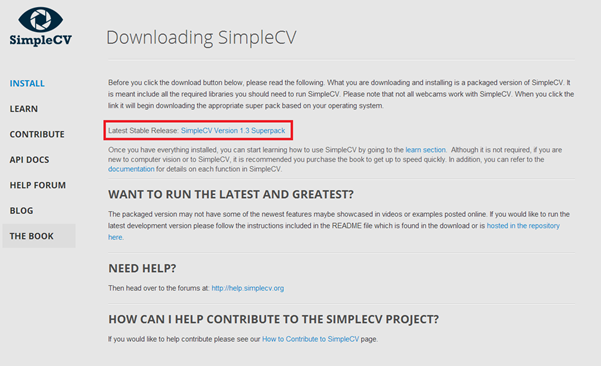
\includegraphics[scale=0.7]{../shared_assets/screenshots/manual/simplecv_download.png}
        \end{figure}

        \paragraph{Linux}
        \begin{enumerate}
            \item Install required system packages for your system using aptitude with the command given below.

            \textit{sudo apt-get install ipython python-opencv python-scipy python-numpy python-pygame python-setuptools python-pip}

            \item Install required packages for Python.

            \textit{sudo pip install SimpleCV svgwrite}

            \item Check the installation was successful. As shown in figure~\ref{fig:simplecvcheck}, this shows that the command ran
            without error.

            \textit{python -c `import SimpleCV'}
            \begin{figure}[H]
                \centering
                \caption{Example of command running without failure.}
                \label{fig:simplecvcheck}
                    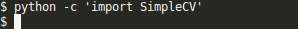
\includegraphics[scale=0.6]{../shared_assets/screenshots/manual/pychecksimplecv.png}
            \end{figure}

            \item Check that the camera is being detected by SimpleCV by running Python, importing SimpleCV and instantiating a 
            Camera object without error. As shown in figure~\ref{fig:cameracheck}.

            \begin{figure}[H]
                \centering
                \caption{Instantiating a Camera object.}
                \label{fig:cameracheck}
                    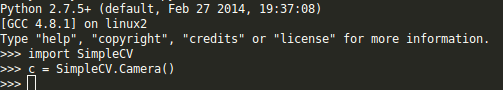
\includegraphics[scale=0.6]{../shared_assets/screenshots/manual/pycheckcamera.png}
            \end{figure}

            \item Add required users by entering the client directory at `code/client' and run the following: \newline
            \textit{python client.py adduser $<$username$>$} \newline
            This should create the directories and take a picture of your face when it is in the frame of the camera. It will have
            created a user when there is a `$<$username$>$.jpg' file in the data folder.

        \end{enumerate}
        \textit{Instructions on how to install SimpleCV on other operating systems can be found here: \url{https://github.com/sightmachine/SimpleCV/blob/master/README.markdown}.}

        \paragraph{Settings}\mbox{}\\
            The files included with the downloaded repository will include an example configuration file called `client.cfg'. As shown
            below in figure~\ref{lst:clientcfg}, this must but set to use values that suite your system needs. To find the `haar\_cascade'
            path you must find where your Python installation resides and check `dist-packages' for the `SimpleCV' folder, then it should
            be under `Features/HaarCascades' as of version 1.3. \newline
            \textit{host} should be the local IP address of the server. \newline
            \textit{port} should be the port the server is running on, which is also defined in the `server.cfg'.

            \begin{figure}[H]
                \centering
                \caption{Example client configuration included in code repository.}
                \label{lst:clientcfg}
                    \lstinputlisting{../../code/client/client.cfg}
            \end{figure}

    \subsubsection{Server}
        The server needs to be installed on a computer that will be up all of the time, this is because people need to be able to access
        the alarm system any time of the day.

        \paragraph{Linux}

        \begin{enumerate}
            \item Install required system packages using aptitude with the command given below.

            \textit{sudo apt-get install python-setuptools python-pip}

            \item Install Twisted Python package.

            \textit{sudo pip install twisted}

            \item Check the Twisted installation, as shown below in figure~\ref{fig:twistedcheck}.

            \textit{python -c `import twisted'}
            \begin{figure}[H]
                \centering
                \caption{Example of command running without failure.}
                \label{fig:twistedcheck}
                    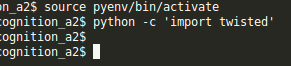
\includegraphics[scale=0.6]{../shared_assets/screenshots/manual/pychecktwisted.png}
            \end{figure}
        \end{enumerate}

        \paragraph{Settings}\mbox{}\\
        The servers settings are all stored in a file called `server.cfg', these are shown in figure~\ref{lst:servercfg}. It isn't
        necessary to change these, only unless something is already running on the port given by default.

        \begin{figure}[H]
            \centering
            \caption{Example client configuration included in code repository.}
            \label{lst:servercfg}
                \lstinputlisting{../../code/server/server.cfg}
        \end{figure}

    \subsection{Database Browser}
        \paragraph{Linux}\mbox{}\\
        \begin{enumerate}
            \item Install system and Python packages using aptitude with the command given below.

            \textit{sudo apt-get install libqt4-sql-sqlite python-qt4 python-qt4-sql}

            \item Once these packages have finished installing, try and run the `db\_browser.pyw' file with `\textit{python db\_browser.pyw}'.
            A window should pop-up as shown in figure~\ref{fig:dbbrowserrun}.

            \begin{figure}[H]
                \centering
                \caption{Example of the Database Browser running.}
                \label{fig:dbbrowserrun}
                    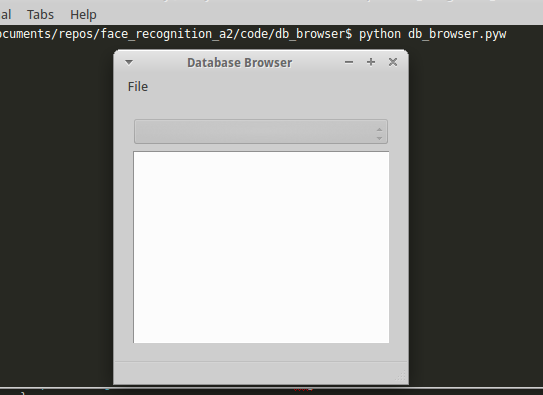
\includegraphics[scale=0.6]{../shared_assets/screenshots/manual/dbbrowserrun.png}
            \end{figure}
        \end{enumerate}

\section{Tutorial}

    \subsection{Introduction}
        I will break down how to use each part of the system in the sections below, each sub-section will include one feature of
        the system explained with detailed text instructions and annotated diagrams to assist you in running the system to its full extent.

    \subsection{Assumptions}
        Assumptions have been made around the proficiency of the user, these include knowing how to start a Python script and having a lot of
        experience previously working with computers.

    \subsection{How to start the server}
        To run the server you must be in the `code/server/' directory and run `\textit{python main.py}'. In figure~\ref{fig:serverrun} you can 
        see the server successfully running.
        \begin{figure}[H]
            \centering
            \caption{Example of the server running.}
            \label{fig:serverrun}
                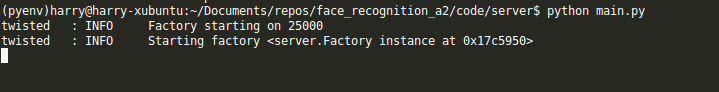
\includegraphics[scale=0.6]{../shared_assets/screenshots/manual/serverrun.png}
        \end{figure}


    \subsection{Running the server as a daemon}
        Running the server as a daemon requires a shell window manager, this keeps a process running which will otherwise be quit when the user
        logs out of the SSH protocol. An example of a suitable window manager is `screen', to install this on Linux you can run 
        `\textit{sudo apt-get install screen}', once installed correctly you can follow the steps below to run the server as a daemon.
        \begin{enumerate}
            \item Run `\textit{screen -S face-server}'.

            This'll spawn a `screen' in which will persist even when the user has logged out of the shell, however your shell will look no different
            apart from being cleared from previous text. To exit this screen you can type `\textit{exit}' while attached to the screen which will terminate
            it. Otherwise, you can hold the \textit{CTRL+A+D} keyboard combination; this'll detach you from the screen, once detached you can reattach to 
            the screen by typing `\textit{screen -r face-server}'.

            \begin{figure}[H]
                \centering
                \caption{Example of `screen' commands.}
                \label{fig:screen}
                    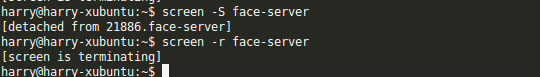
\includegraphics[scale=0.6]{../shared_assets/screenshots/manual/screen.png}
            \end{figure}

            \item While in the `server' directory of the repository run `\textit{python main.py}', and you can then detach from this by using the steps
            explained in step 1.

        \end{enumerate}

    \subsection{How to start the client}
        To run the client you must be in the `code/client/' directory and run `\textit{python client.py}'. In figure~\ref{fig:clientrun} you can 
        see the client successfully running.
        \begin{figure}[H]
            \centering
            \caption{Example of the client running.}
            \label{fig:clientrun}
                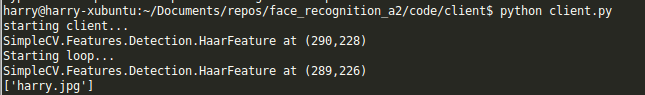
\includegraphics[scale=0.6]{../shared_assets/screenshots/manual/clientrun.png}
        \end{figure}


    \subsection{How to start the database browser}
        To run the database browser you must be in the `code/db\_browser/' directory and run `\textit{python db\_browser.pyw}'. In figure~\ref{fig:dbbrowserrun} you can 
        see the database browser successfully running.

    \subsection{How do I create a new user?}
        This requires actions on both the server and client, firstly the user must be added to the server database so that the client request 
        succeeds when prompted. This requires running the `db\_browser' and adding a user via the provided user interface, in figure~\ref{fig:dbadduser}
        you can see the `File' menu being opened and a new user dialogue popping up.

        \begin{figure}[H]
            \centering
            \caption{Example of new user dialog.}
            \label{fig:dbadduser}
                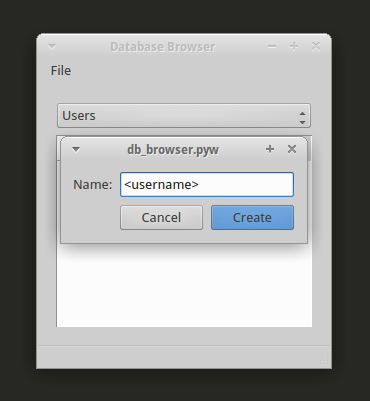
\includegraphics[scale=0.7]{../shared_assets/screenshots/manual/dbadduser.png}
        \end{figure}

        Secondly, a user must be added to the client, this can be done by facing the user in front of the camera and running `\textit{python client.py adduser $<$name$>$}',
        or images with the face of the user cropped can be added to the `client/data/usr' folder with $<$name$>$.jpg naming convention.
    \newpage
    \subsection{How do I start a new log file?}
        To create a new log you simply select File $>$ New $>$ Log File, from the Database Browser, as shown in figure~\ref{fig:dbaddlog}.

        \begin{figure}[H]
            \centering
            \caption{File $>$ New Menu}
            \label{fig:dbaddlog}
                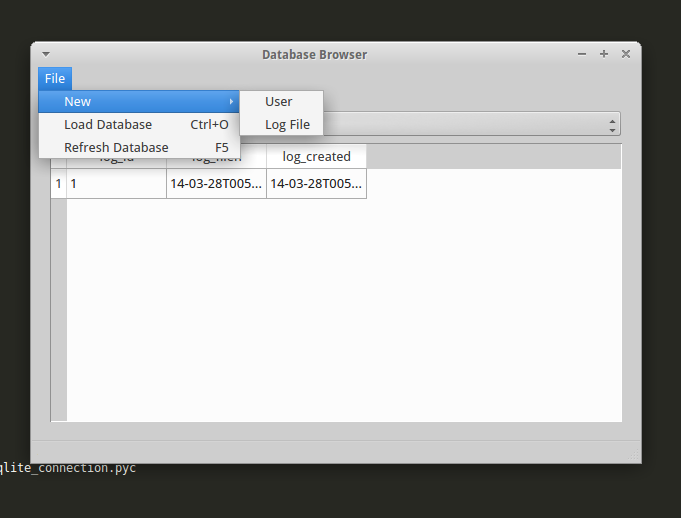
\includegraphics[scale=0.5]{../shared_assets/screenshots/manual/dbaddlog.png}
        \end{figure}        


\section{Errors}
    \subsection{SimpleCV/Camera related}
        \begin{figure}[H]
            \centering
            \caption{Example of a camera not found error}
            \label{fig:camera404}
                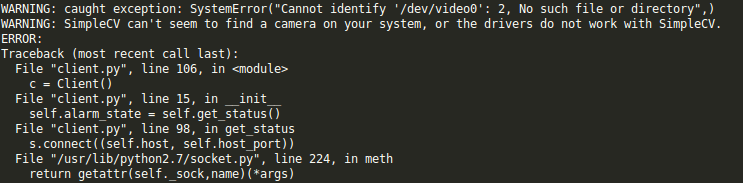
\includegraphics[scale=0.5]{../shared_assets/screenshots/manual/camera404.png}
        \end{figure} 
        This error will occur to the client when a camera has not been detected by SimpleCV, to fix this you can follow the steps below:
        \begin{enumerate}
            \item Check the camera is connected to the client computer
            \item Check the camera's drivers are installed
            \item Try a different USB port
        \end{enumerate}



    \subsection{Network related}
        \begin{figure}[H]
            \centering
            \caption{Example of a network error}
            \label{fig:networkcrash}
                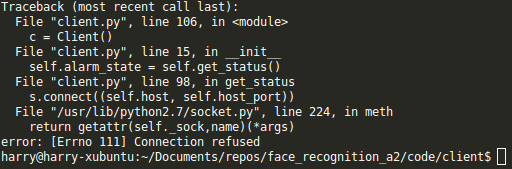
\includegraphics[scale=0.5]{../shared_assets/screenshots/manual/networkcrash.png}
        \end{figure} 
        This error will occur to the client file when it cannot reach the server, this is because when the client is initially started the 
        server is queried by the client and when the client cannot connect to the given port, this error is raised. To fix this you either
        need to:
        \begin{enumerate}
            \item Check the server is running, if not start it
            \item Check the client is pointed towards the right socket
            \item Check the client or server have access to the local area network
        \end{enumerate}

    \subsection{Database}
        \begin{figure}[H]
        \centering
        \caption{Example of a database error}
        \label{fig:db404}
            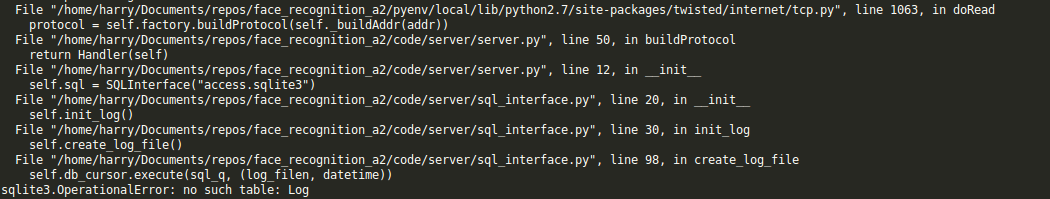
\includegraphics[scale=0.4]{../shared_assets/screenshots/manual/db404.png}
    \end{figure} 
    This error will occur to the server when the database has not been initialised; this means that the SQLite database probably doesn't exist.
    To fix this you should run `python sql\_interface.py' to initialise the database, if this doesn't work then you can check the following:
    \begin{enumerate}
        \item Check the database is located in the same folder as `server.py'
        \item Check the database file hasn't been renamed
    \end{enumerate}
\newpage
\section{System Recovery}
    \newpage
    \subsection{Backing up data}
        \subsubsection{Client}
            \begin{enumerate}
                \item Compress the `data' folder within the client folder.
                \begin{center}
                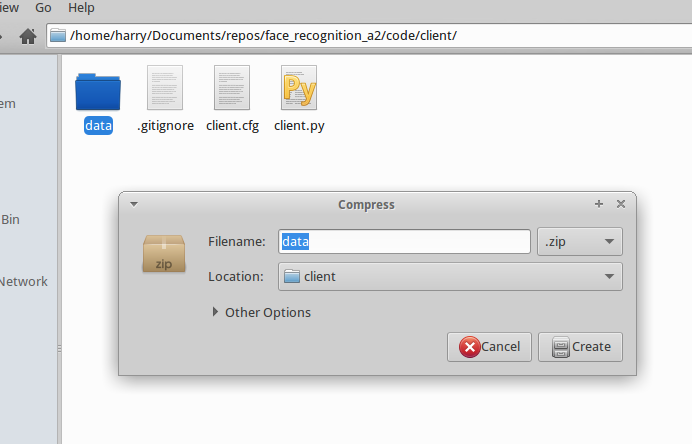
\includegraphics[scale=0.4]{../shared_assets/screenshots/manual/compressclientdata.png}
                \end{center}
                \item Store this compressed copy of the folder on a different medium, such as USB
                \begin{center}
                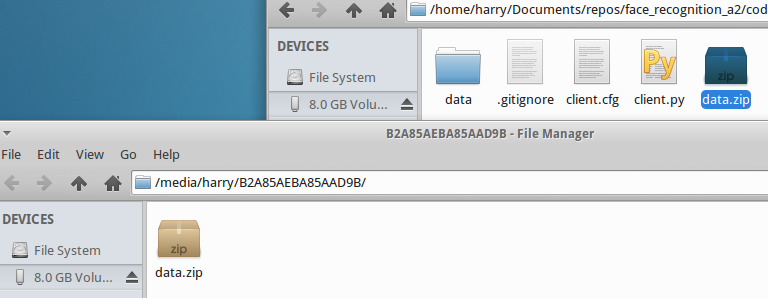
\includegraphics[scale=0.4]{../shared_assets/screenshots/manual/clientstoredusb.png}
                \end{center}
            \end{enumerate}
            All of the sensitive data stored on the client are now backed up in a different medium or folder.
        \newpage
        \subsubsection{Server}
            \begin{enumerate}
                \item Compress the `logs' folder within the client folder.
                \begin{center}
                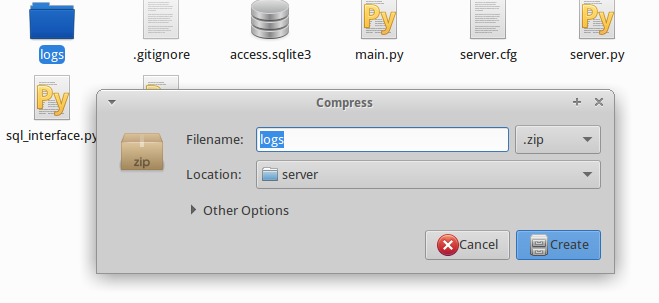
\includegraphics[scale=0.4]{../shared_assets/screenshots/manual/compressserverdata.png}
                \end{center}
                \item Store this compressed copy of the folder and the `access.sqlite3' file on a different medium, such as USB
                \begin{center}
                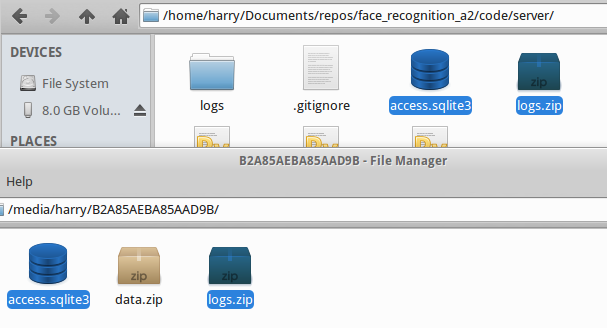
\includegraphics[scale=0.4]{../shared_assets/screenshots/manual/serverstoredusb.png}
                \end{center}
            \end{enumerate}
            All of the sensitive data stored on the server are now backed up in a different medium or folder.

    \subsection{Restoring data}
        \subsubsection{Client}
            \begin{enumerate}
                \item Decompress the backed up `data' zip.
                \begin{center}
                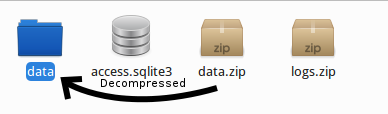
\includegraphics[scale=0.7]{../shared_assets/screenshots/manual/decompressedclient.png}
                \end{center}
                \item Delete the pre-existing data folder, if it exists, in the client folder.
                \begin{center}
                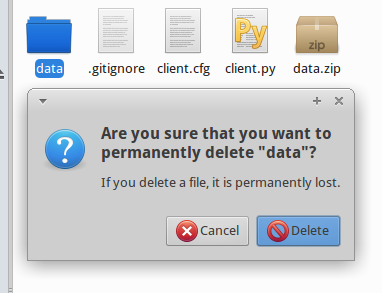
\includegraphics[scale=0.7]{../shared_assets/screenshots/manual/deleteclientdata.png}
                \end{center}
                \item Move this back up uncompressed data folder back into the client folder.
                \begin{center}
                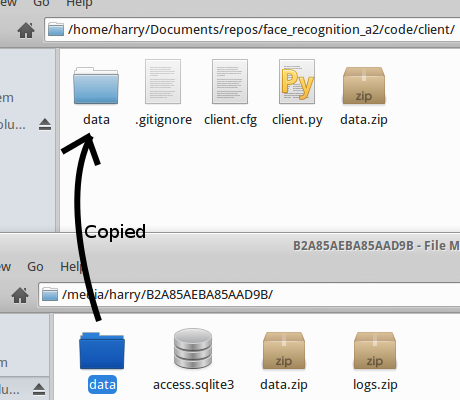
\includegraphics[scale=0.6]{../shared_assets/screenshots/manual/restoreclient.png}
                \end{center}
            \end{enumerate}
            The client will now be restored to the latest back up.
        \newpage
        \subsubsection{Server}
            \begin{enumerate}
                \item Overwrite the existing `access.sqlite3' with the backed up version.
                \begin{center}
                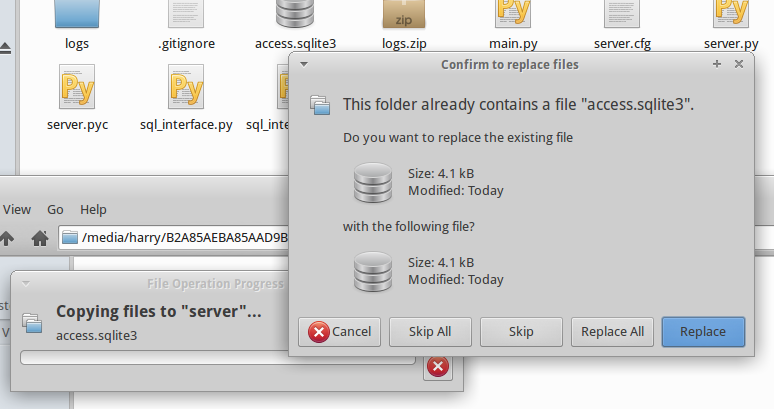
\includegraphics[scale=0.5]{../shared_assets/screenshots/manual/serveroverwritedb.png}
                \end{center}
                \item Delete the pre-existing `logs' folder, if it exists, in the server folder.
                \begin{center}
                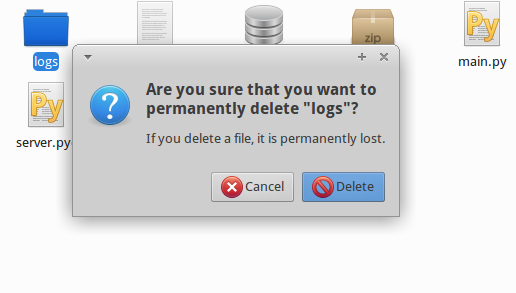
\includegraphics[scale=0.7]{../shared_assets/screenshots/manual/serverlogdelete.png}
                \end{center}
                \item Decompress the backed up `logs' folder.

                \item Move this back up uncompressed logs folder back into the server folder.
                \begin{center}
                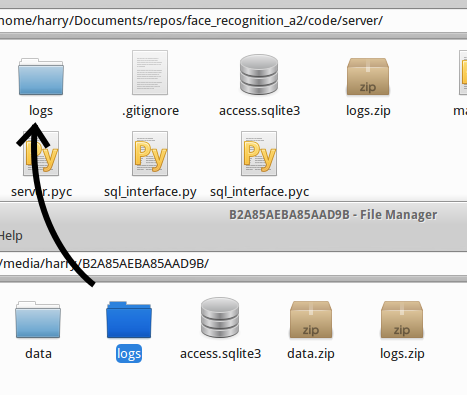
\includegraphics[scale=0.6]{../shared_assets/screenshots/manual/serverlogmove.png}
                \end{center}
            \end{enumerate}

\end{document}